\documentclass[authoryear]{elsarticle}
\usepackage{latexsym}
%\usepackage{rotate}
\usepackage{graphics}
\usepackage{amsmath}
\usepackage{amssymb}
\usepackage{comment}
\bibliographystyle{chicago}



\newcommand{\logit}{\mathrm{logit}}
\newcommand{\I}{\mathrm{I}}
\newcommand{\E}{\mathrm{E}}
\newcommand{\p}{\mathrm{P}}
\newcommand{\e}{\mathrm{e}}
\newcommand{\vecm}{\mathrm{vec}}
\newcommand{\kp}{\otimes}
\newcommand{\diag}{\mathrm{diag}}
\newcommand{\cov}{\mathrm{cov}}
\newcommand{\eps}{\epsilon}
\newcommand{\ep}{\varepsilon}
\newcommand{\obdots}{\ddots}    % change this later
\newcommand{\Ex}{{\cal E}}
\newcommand{\rat}{{\frac{c_{ij}}{c_{i,j-1}}}}
\newcommand{\rmu}{m}
\newcommand{\rsig}{\nu}
\newcommand{\fd}{\mu}
\newcommand{\tr}{\mathrm{tr}}
\newcommand{\cor}{\mathrm{cor}}
\newcommand{\bx}[1]{\ensuremath{\overline{#1}|}}
\newcommand{\an}[1]{\ensuremath{a_{\bx{#1}}}}

\newcommand{\bi}{\begin{itemize}}
\newcommand{\ei}{\end{itemize}}

\renewcommand{\i}{\item}
\newcommand{\sr}{\ensuremath{\mathrm{SRISK}}}
\newcommand{\cs}{\ensuremath{\mathrm{CS}}}
\newcommand{\cri}{\ensuremath{\mathrm{Crisis}}}
\newcommand{\var}{\ensuremath{\mathrm{VaR}}}
\newcommand{\covar}{\ensuremath{\mathrm{CoVaR}}}
\newcommand{\med}{\ensuremath{\mathrm{m}}}
\newcommand{\de}{\mathrm{d}}
\renewcommand{\v}{\ensuremath{\mathrm{v}_q}}
\newcommand{\m}{\ensuremath{\mathrm{m}}}
\newcommand{\tvar}{\ensuremath{\mathrm{TVaR}}}



\newcommand{\eref}[1]{(\ref{#1})}
\newcommand{\fref}[1]{Figure \ref{#1}}
\newcommand{\sref}[1]{\S\ref{#1}}
\newcommand{\tref}[1]{Table \ref{#1}}
\newcommand{\aref}[1]{Appendix \ref{#1}}




\newcommand{\cq}{\ , \qquad}
\renewcommand{\P}{\mathrm{P}}
\newcommand{\Q}{\mathrm{Q}}

\newcommand{\Vx}{{\cal V}}
\newcommand{\be}[1]{\begin{equation}\label{#1}}
\newcommand{\ee}{\end{equation}}




\begin{document}

% Title of paper
\title{Systemic risk and contagion effects in Australian financial institutions and sectors}
% List of authors, with corresponding author marked by asterisk
\author{Piet de Jong,  Geoff Loudon and Weihao Choo \\[4pt]
% Author addresses
\textit{Department of Applied Finance and Actuarial Studies\\ Macquarie University, Sydney, NSW 2109.}
\\[2pt]
%E-mail address for correspondence
{piet.dejong@mq.edu.au}}

% Running headers of paper:
\markboth%
% First field is the short list of authors
{De Jong}
% Second field is the short title of the paper
{Systemic risk}

\maketitle


\section{Joint model}

Suppose the market return is $r_m$ with stationary distribution function $F_m$ and percentile rank $u_m\equiv F_m(r_m)$. Hence $u_m$ is uniform over the unit interval in stationarity. In addition the return of stock $i$ is $r_i$ with percentile rank $u_i\equiv F_i(r_i)$ where $F_i$ is the stationary distribution function. There are $n$ stocks forming the market: $i=1,\ldots, n$. In addition the joint distribution of $(u_m,u_i)$ is $C_i$, a copula. Returns of individual stocks are partly driven by the market, known as systematic risk in the capital asset pricing model.
\newline

It is well known that stock returns in the short term exhibit behaviour such as volatility clustering and varying dependence. This behaviour is captured by assuming $u_m$ is a time series, or $u_{m,t}$, deviating away from uniformity in the short term but attaining uniformity in stationarity. Given $u_{m,t}$,  market return is $r_{m,t}=F_m^-(u_{m,t})$. In addition $u_{i,t}$ is drawn from the conditional distribution $C_i(u_i|u_m)$ and the return on stock $i$ is $r_{i,t}=F_i^-(u_{i,t})$. Similar to $u_{m,t}$, $(r_{m,t},r_{i,t})$ deviates from its stationary joint distribution in the short term.
\newline

Assume:
\bi
\i $F_m$ and $F_i$ have fat tails

\i $C_i$ captures positive dependence overall, and strong tail dependence

\i $u_{m,t}$ exhibits volatility clustering, that is sustained periods of stability or volatility, but uniform as $t\rightarrow \infty$.
\ei
The above setup captures stylised features of short term stock returns in the following way:
\bi
\i Fat tail distributions and strong tail dependence give rise to simultaneous extreme stock returns representing market crashes or surges.

\i Volatility clustering of both market and individual stock returns due to positive dependence.

\i Strong inter-stock dependence during market volatility due to tail dependence, and weaker dependence in times of stability.
\ei




\section{Illustration}


Suppose the pseudo market return follows a ARCH(3) process
$$
r_{m,t}=F_m^-\{\p(\tilde{r}_{m,t})\} \cq \tilde{r}_{m,t}=\epsilon_t \sqrt{a+b\tilde{r}_{m,t-1}^2+c\tilde{r}_{m,t-2}^2+d\tilde{r}_{m,t-3}^2} \;,
$$
where $\p$ is the percentile rank transform and $\epsilon_t$ is white noise. Then whilst market return $r_{m,t}$ follows $F_m$ in the long run, there are volatility clusters whereby $r_{m,t}$ is volatile for a sustained period (when $r_{m,t}$ is large) and stable otherwise (when $r_{m,t}$ is small). Assume $a=1$, $b=0.5$, $c=0.3$ and $d=0.2$.
\newline

Consider two stocks. Model the dependence between their returns with the market return using a factor copula
$$
u_{m,t} = \p(f-g+e_m) \cq u_{1,t} = \p(a_1 f-b_1 g+e_1) \cq u_{2,t} = \p(a_2 f-b_2g+e_2) \;,
$$
where $e_m$, $e_1$ and $e_2$ are noise terms, $f$ and $g$ are skewed non-negative random variables, and the other variables are constants. As before $\p$ is the percentile rank transform. The factors $f$ and $g$ induce upper and lower tail dependence between individual and market returns respectively. Assume $f$ and $g$ are exponential with mean one. In addition $a_1=b_1=2$ and $a_2=b_2=2$. Hence $r_2$ has stronger tail dependence between $r_m$. 
\newline

Lastly assume $r_m$, $r_1$ and $r_2$ follow $t_2$ distributions in stationarity. The $t_2$ distribution captures skewed returns captured to the Gaussian.
\newline

The model does not seek to specify the relationship between $r_m$, $r_1$ and $r_2$. In practice the market is formed by a large number of stocks. This model focuses on two stocks in the basket, whilst ignoring others.
\newline

The below figures illustrate the assumed model. Note that the model captures stylised features of stock return.



\begin{figure}
  \begin{center}
    \begin{tabular}{cc}
      \resizebox{60mm}{!}{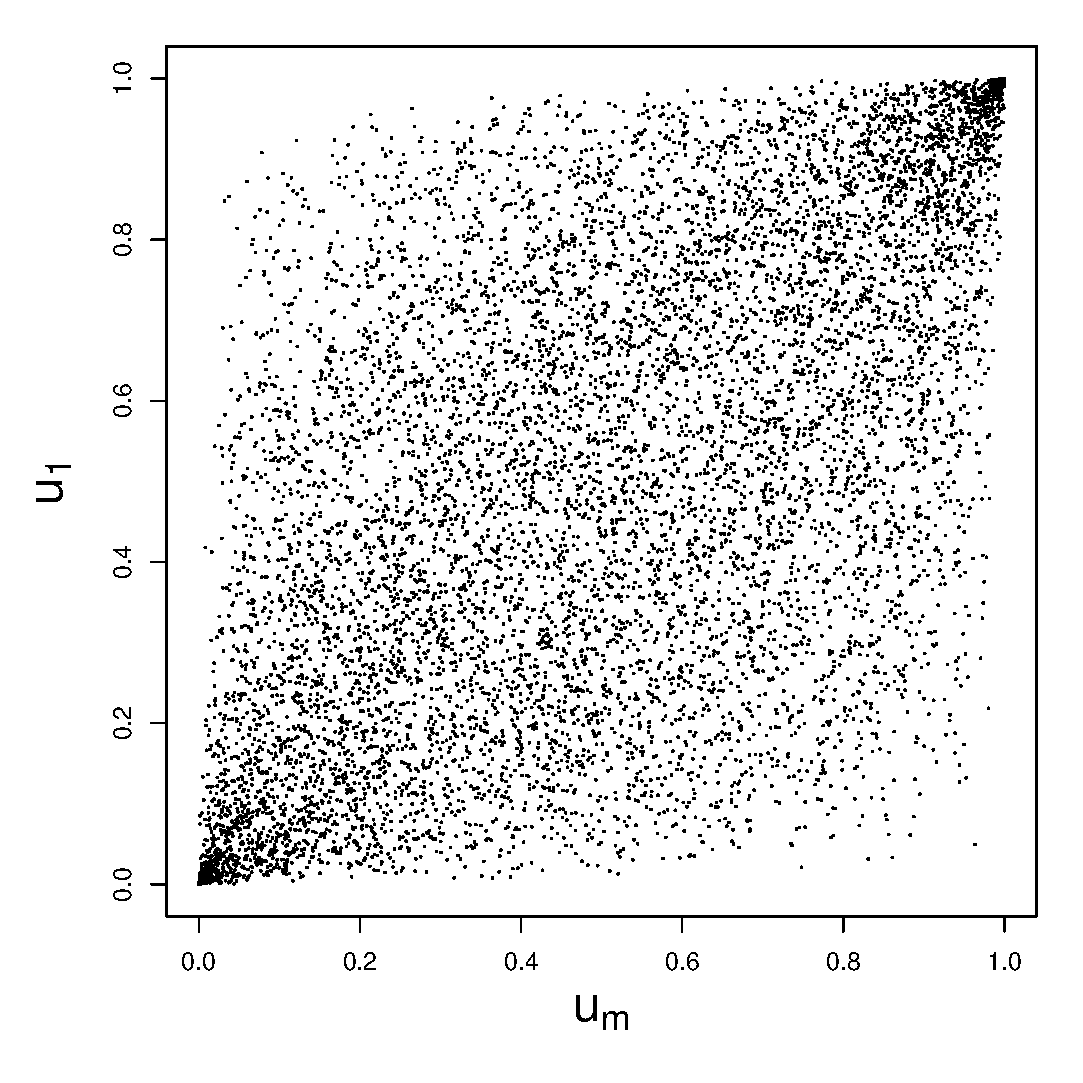
\includegraphics{copula1.eps}}
      \resizebox{60mm}{!}{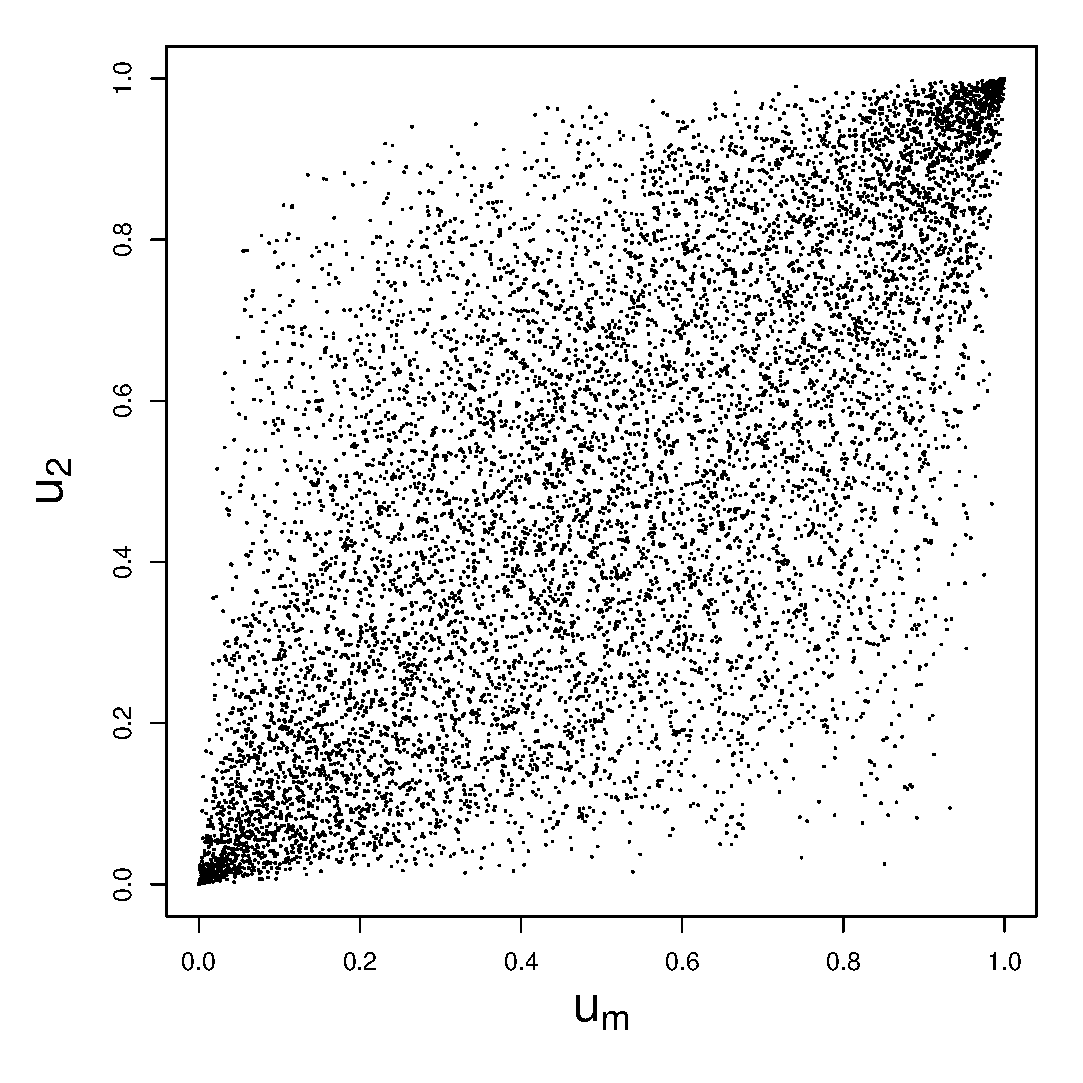
\includegraphics{copula2.eps}} \\
    \end{tabular}
    \caption{Left and right panels  plot 10,000 simulated points of $(u_m,u_1)$ and $(u_m,u_2)$ respectively based on the assumed factor copula. Note the tail dependence.}
    \label{finterpretation}
  \end{center}
\end{figure}


\begin{figure}
  \begin{center}
    \begin{tabular}{c}
      {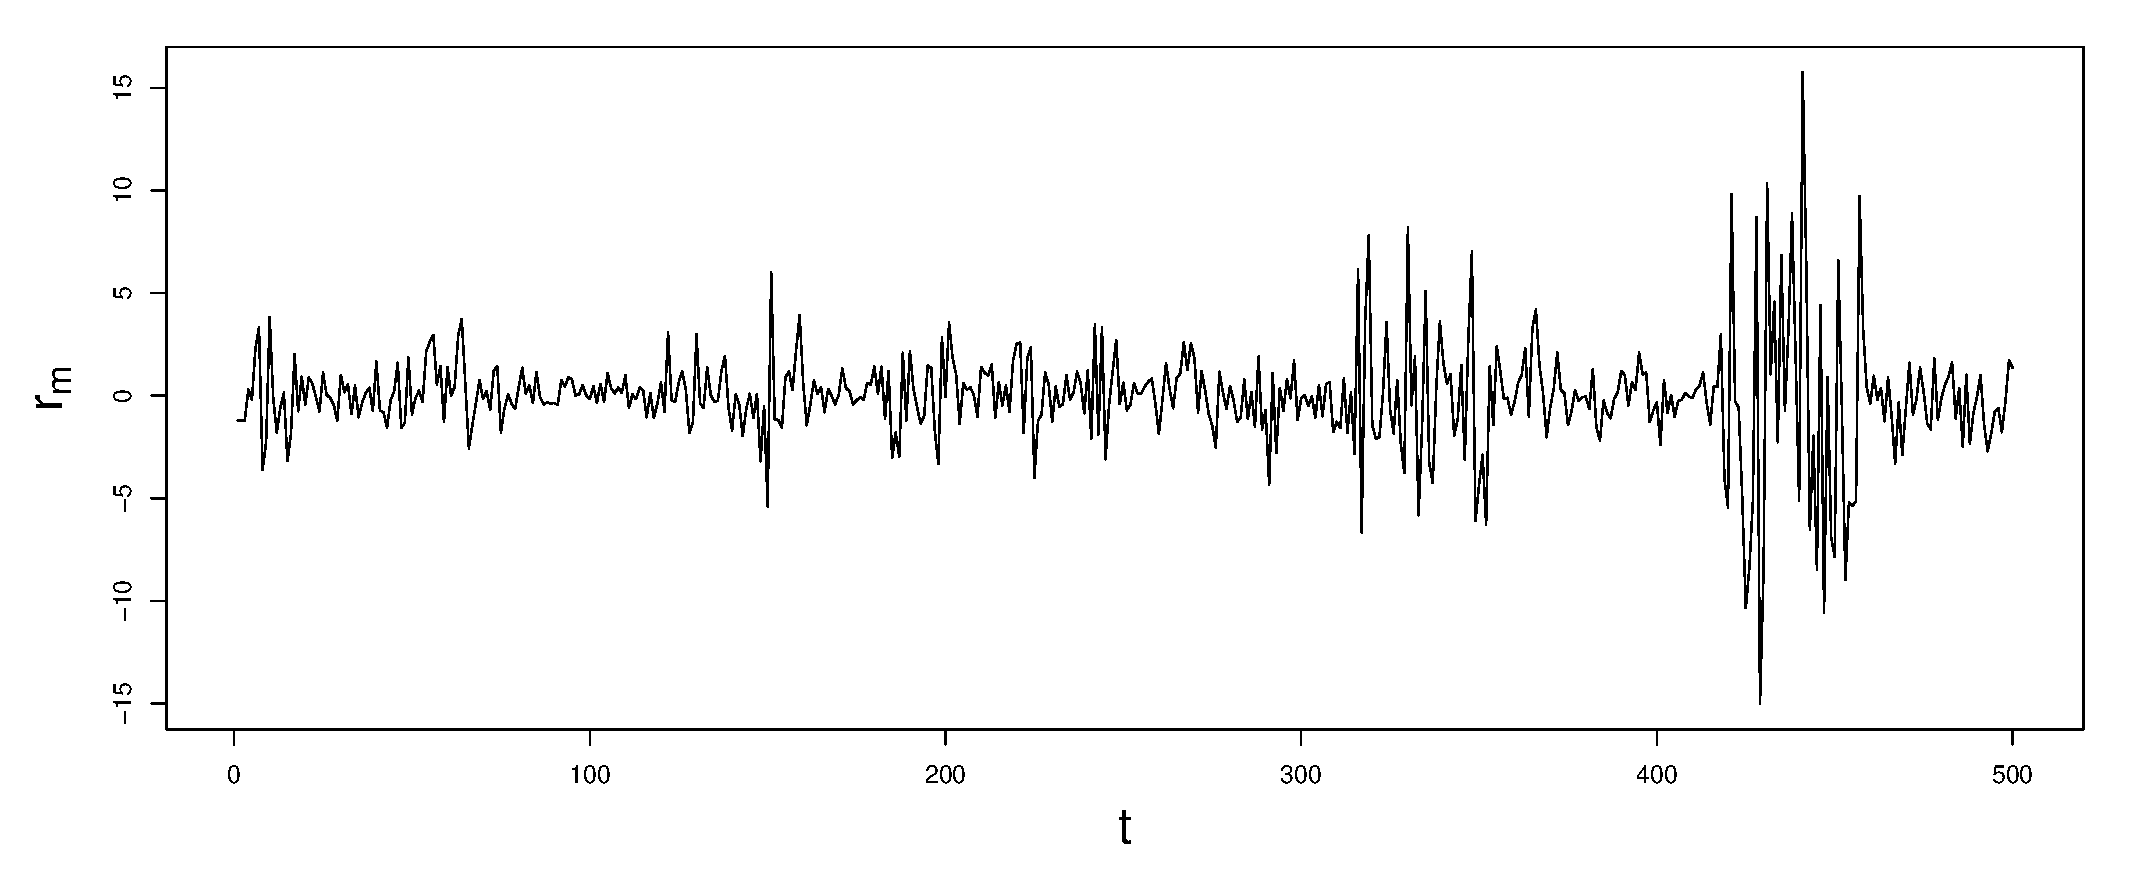
\includegraphics[scale=0.35]{marketreturn.eps}} \\
       {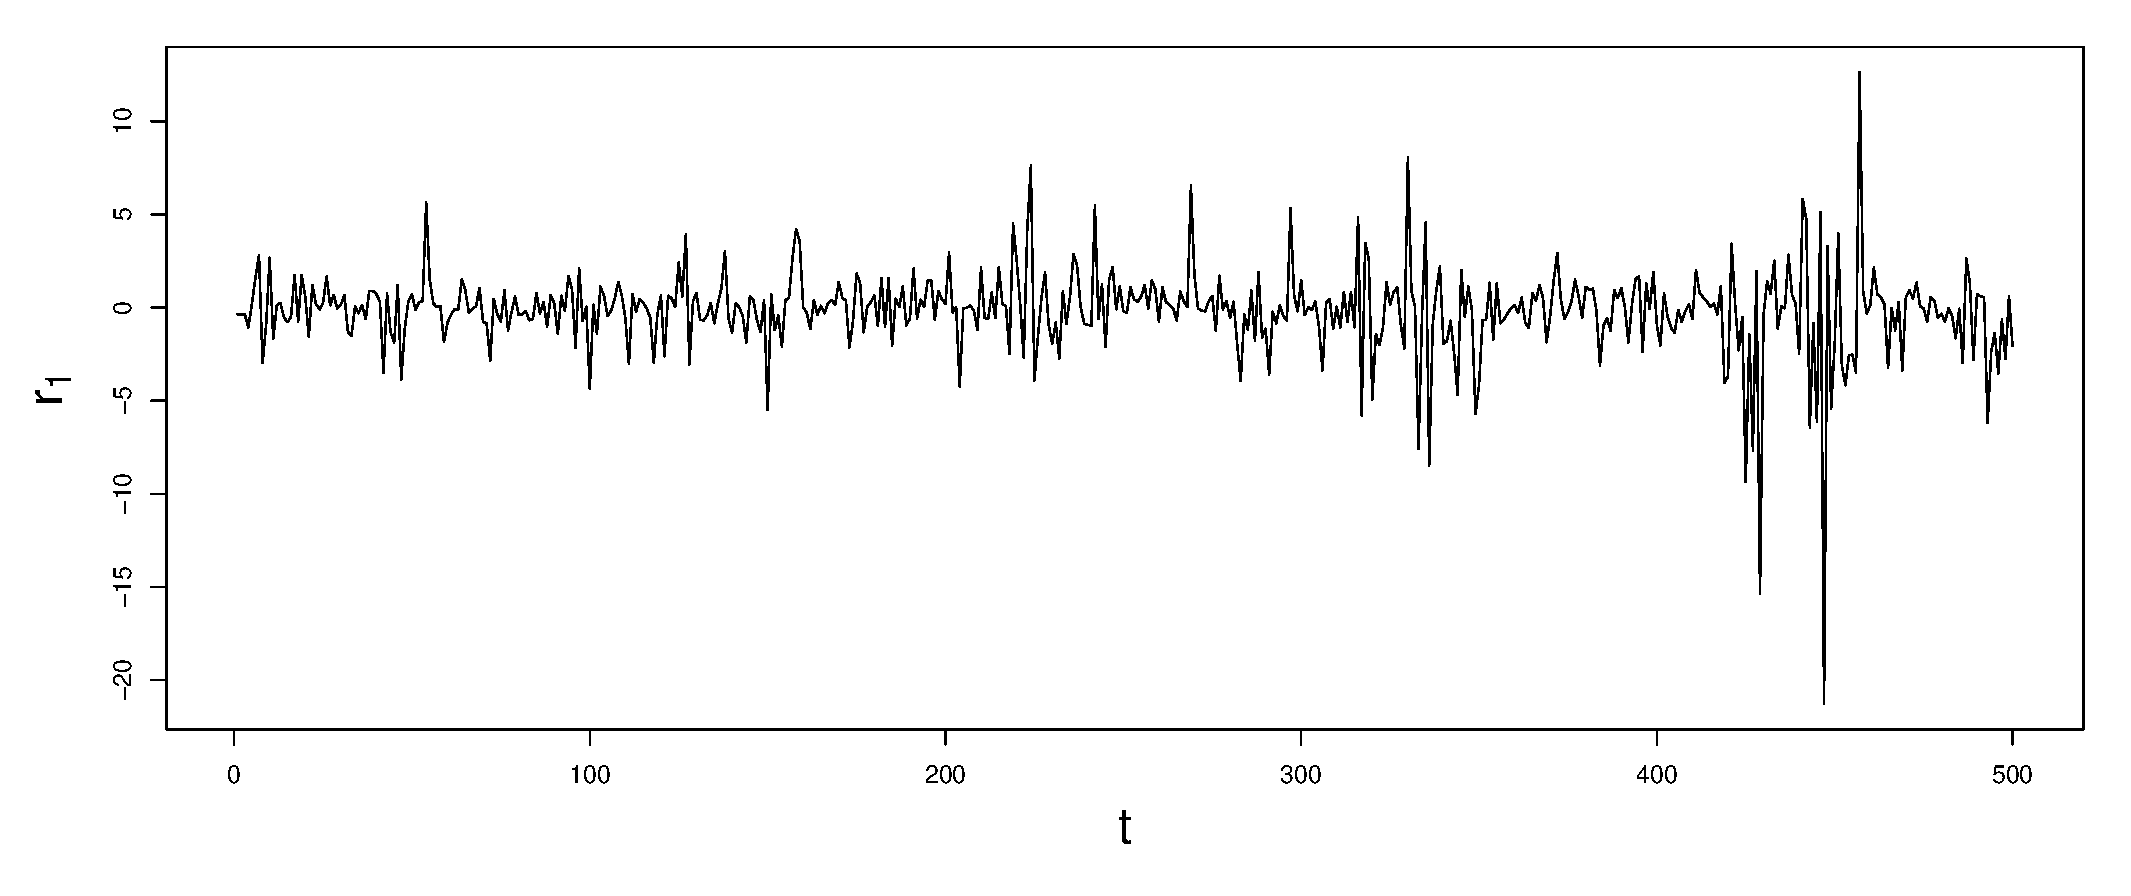
\includegraphics[scale=0.35]{return1.eps}} \\
        {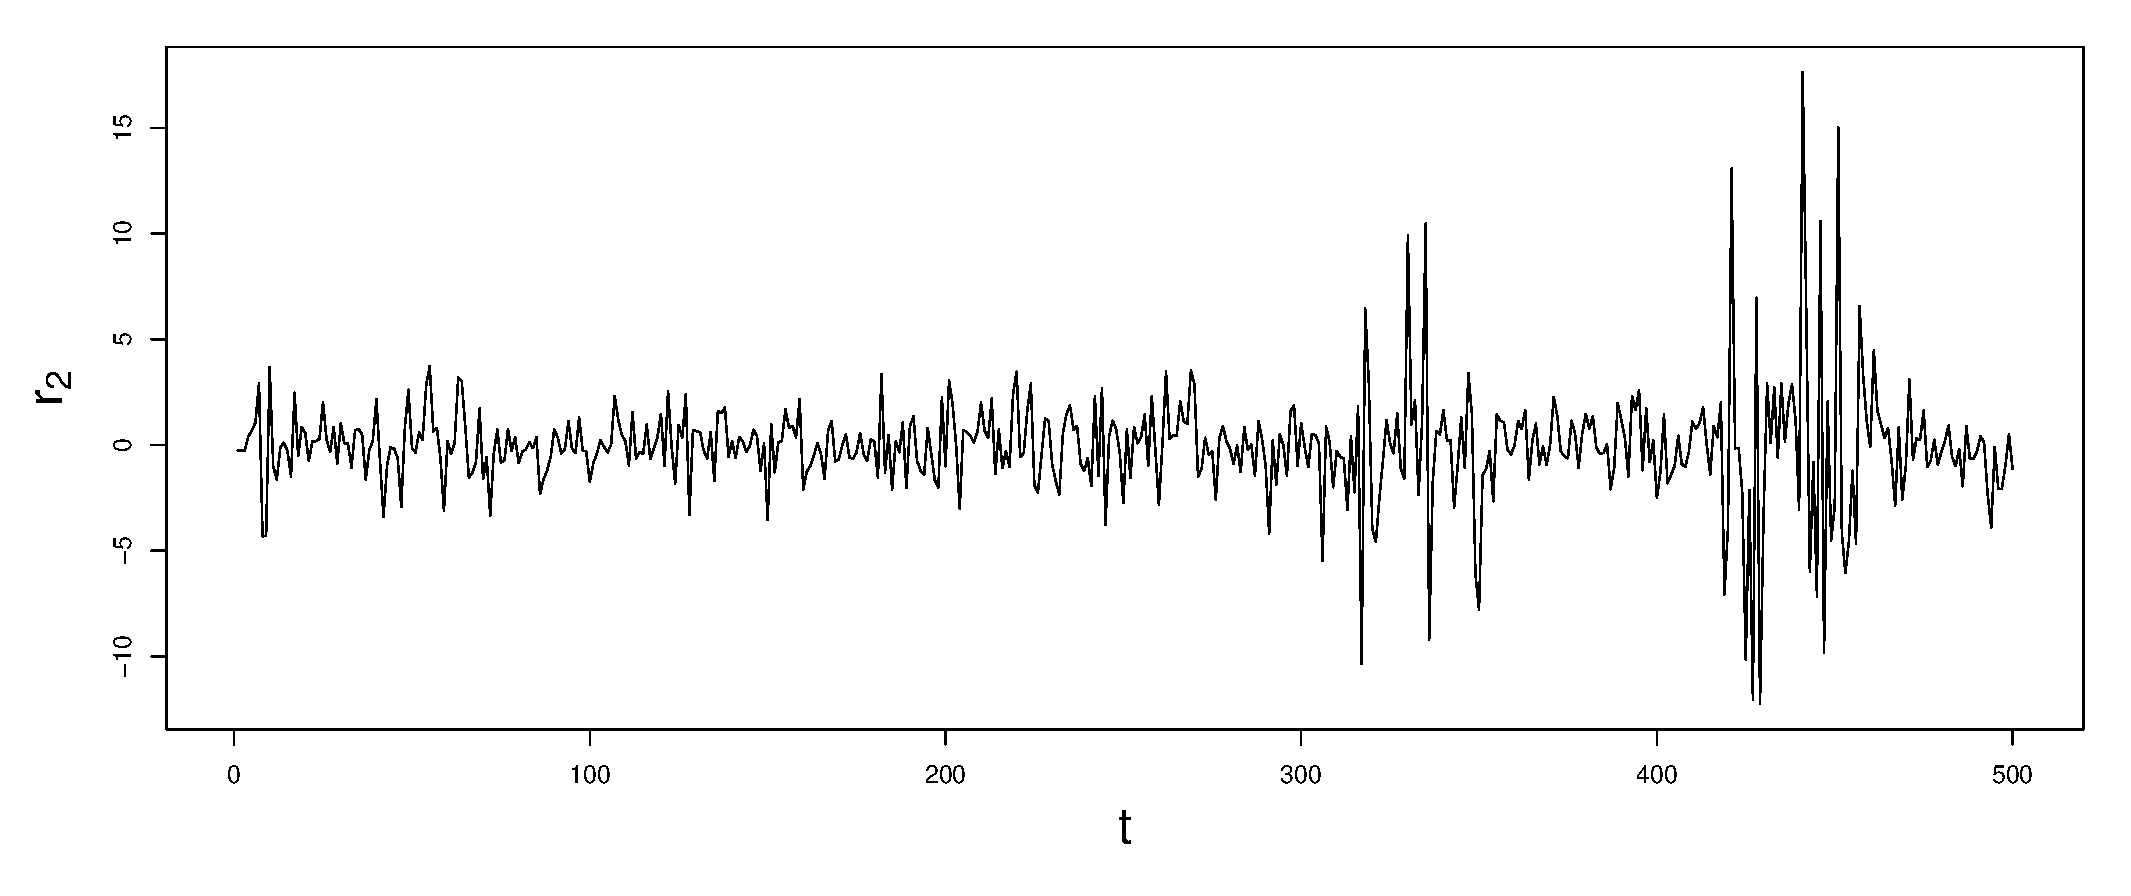
\includegraphics[scale=0.35]{return2.eps}} \\
     \end{tabular}
    \caption{Daily returns $r_{m,t}$ (top panel), $r_{1,t}$ (middle panel) and $r_{2,t}$ (bottom panel). Note the simultaneous volatility clustering in each return.}
    \label{finterpretation}
  \end{center}
\end{figure}



\begin{figure}
  \begin{center}
    \begin{tabular}{c}
      {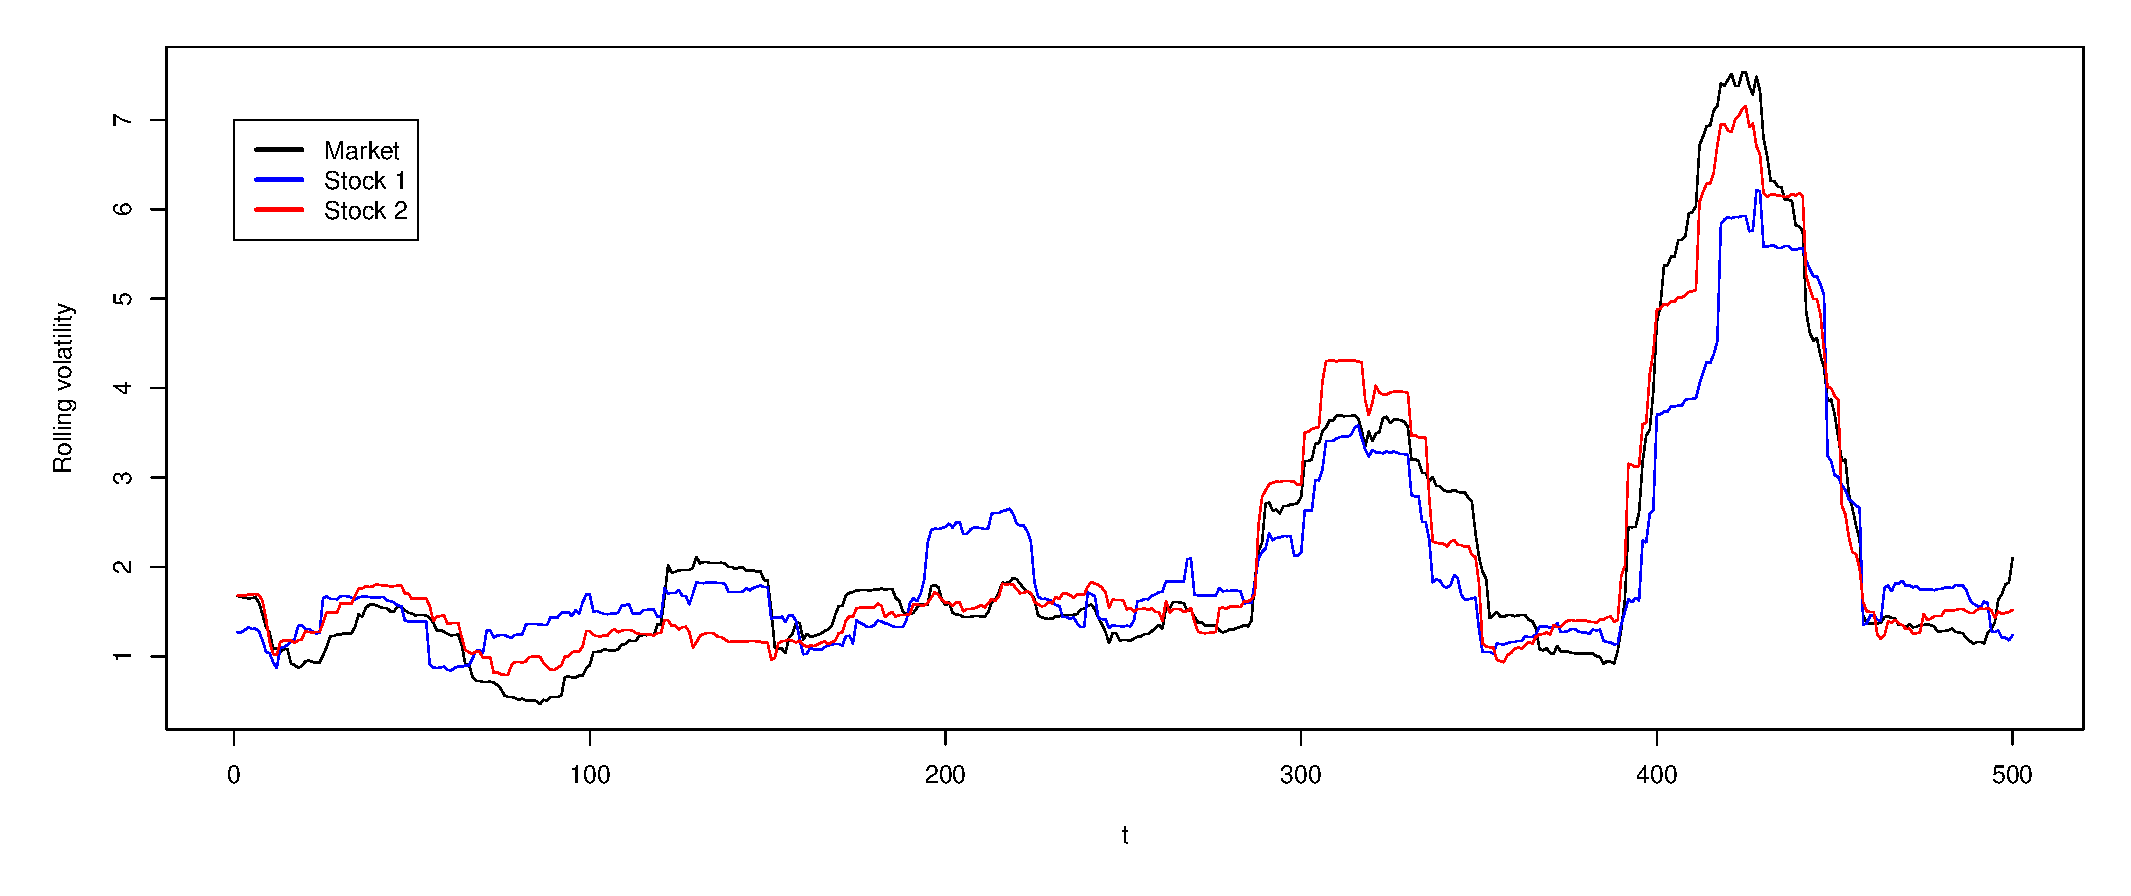
\includegraphics[scale=0.35]{rollingvolatility.eps}} \\
       {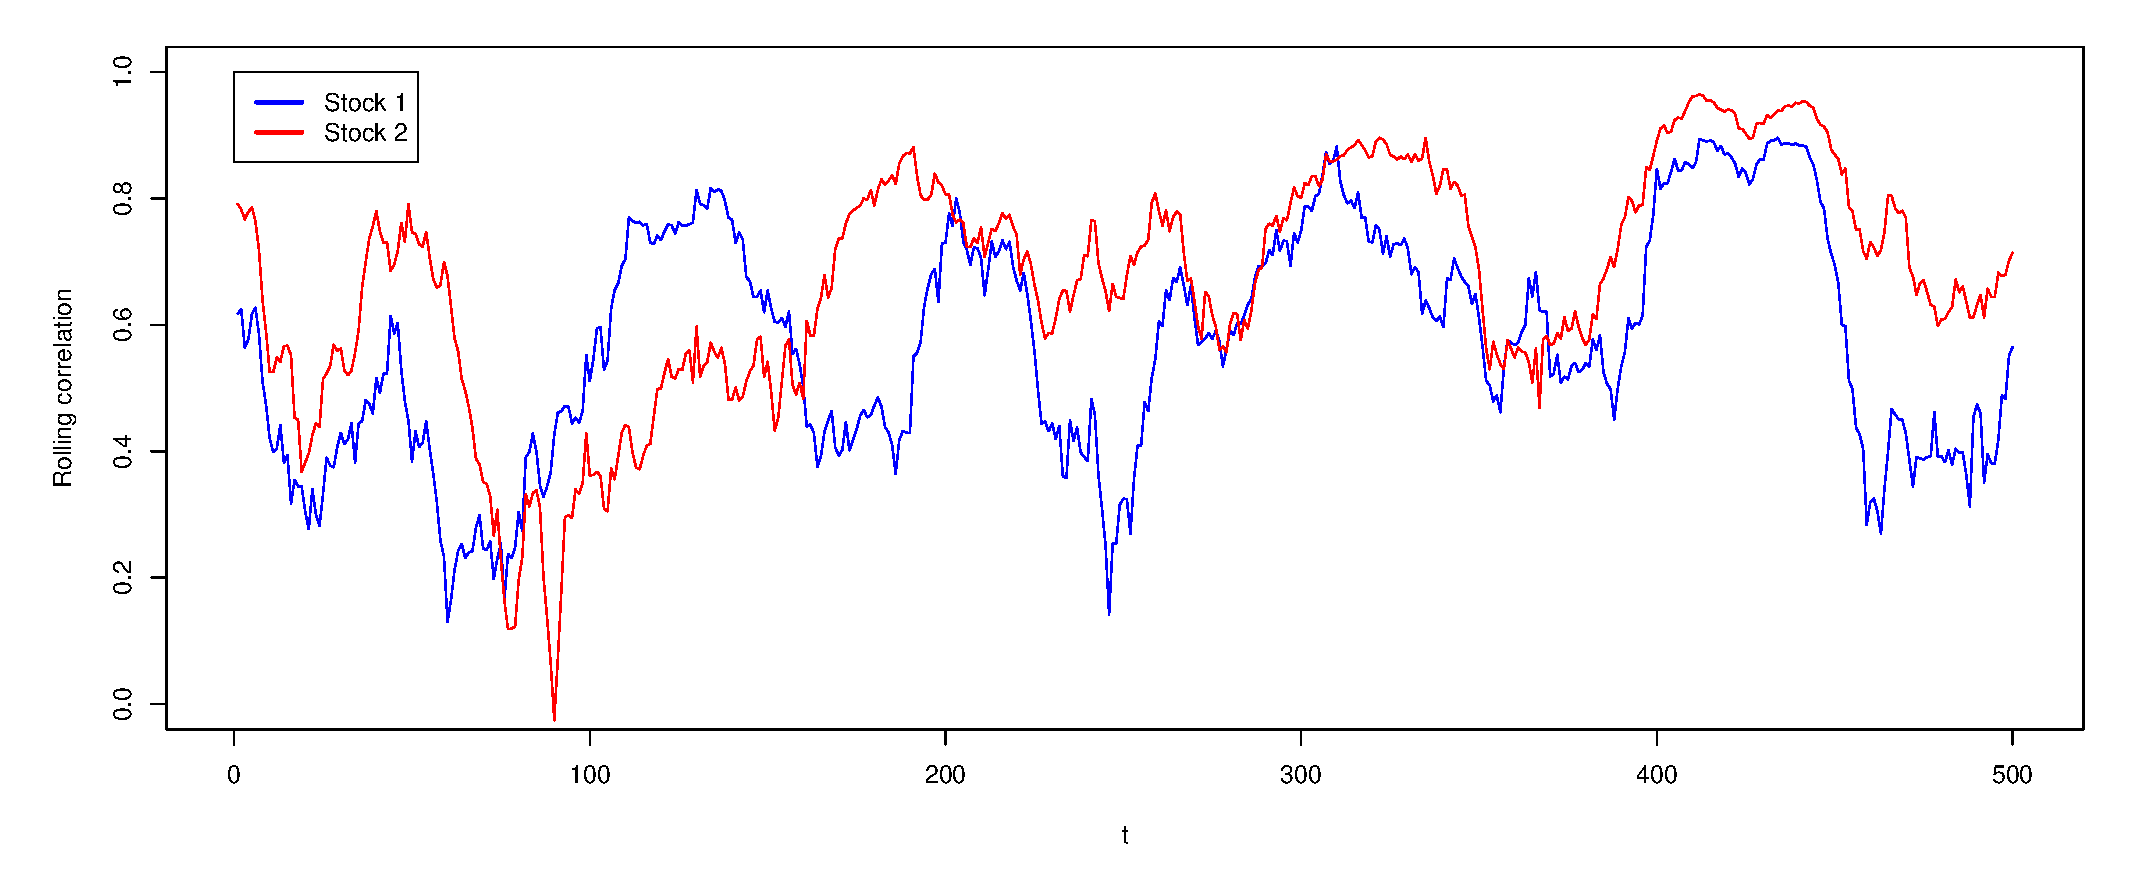
\includegraphics[scale=0.35]{rollingcorrelation.eps}} \\
            \end{tabular}
    \caption{Top panel shows 30-day rolling volatility of $r_{m,t}$, $r_{1,t}$ and $r_{2,t}$. Bottom panel shows 30-day rolling rank correlation for $(r_{m,t},r_{1,t})$ and $(r_{m,t},r_{2,t})$. Note the strong correlations occurring simultaneously with volatility clusters. In addition stock 2 has stronger resemblance with the market.}
    \label{finterpretation}
  \end{center}
\end{figure}





\end{document}
